\section{Laboratory work implementation}

\subsection{Tasks and Points}

- Realizeaza un simplu site; \\
\indent 
- Site-ul trebuie sa contina AJAX Requests; \\
\indent 
- Implimentarea XHR sau JSON responses. Careva din informatie trebuie sa fie dinamic incarcata pe pagina;

\subsection{Analiza lucrarii de laborator}
\selectlanguage{russian}
В ходе данной лабораторной работы был разработан сайт, содержащий информацию из панграмм. Сайт состоит из нескольких страниц первая их которых - index.php - демонстрация использования технологий HTML и CSS, а на последующих находятся: 1)Форма заполняемая пользователем, для загрузки информации о книгах в базу данных; 2)СТраница, реализующая поиск необходимой книги в базе данных; 3)Страница с результатами поиска.\\
\indent 
Созданный сайт имеет связь с базой данных. Используется база данных MySql. Находящаяся на localhost'e, созданном с помощью утилиты denwer.\\
\indent 
Для обеспечения функциональности использовались технологии и языки PHP, HTML, CSS. На языке HTML написаны сами страницы. Для верстки index.php был использован фреймворк 960 grid system. Разметка для второго файла отправляется вместе с файлом main2.php. В файлах .php находятся команды, которые позволяют взаимодействовать с базой данных. В лабораторной работе используются только один тип запросов - POST. \\
\indent 
Коды можно просмотреть на репозитории 



\subsection{Imagini}

\begin{figure}[h]
	\center{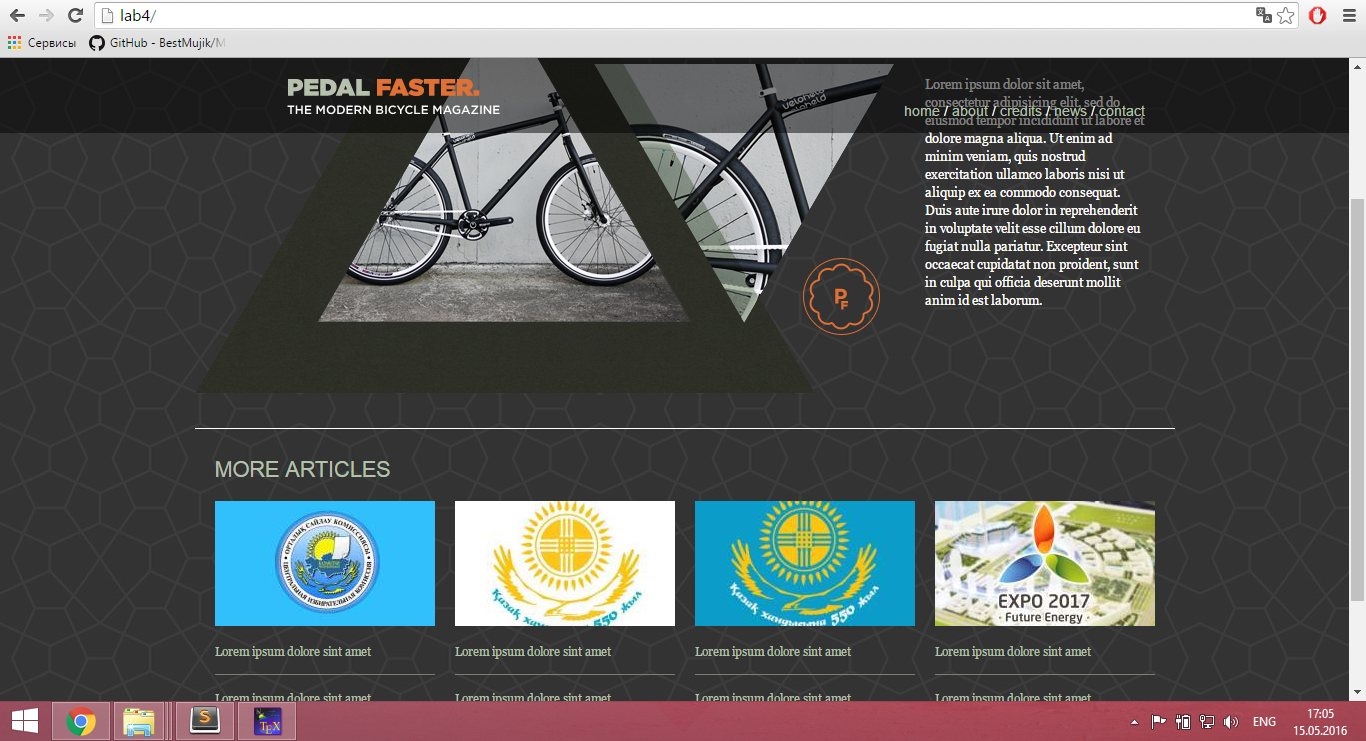
\includegraphics[width=1\linewidth]{images/index.jpg}}
	\caption{Заглавная страница}
	\label{ris:image}
\end{figure}
\hfill
\begin{figure}[h]
	\center{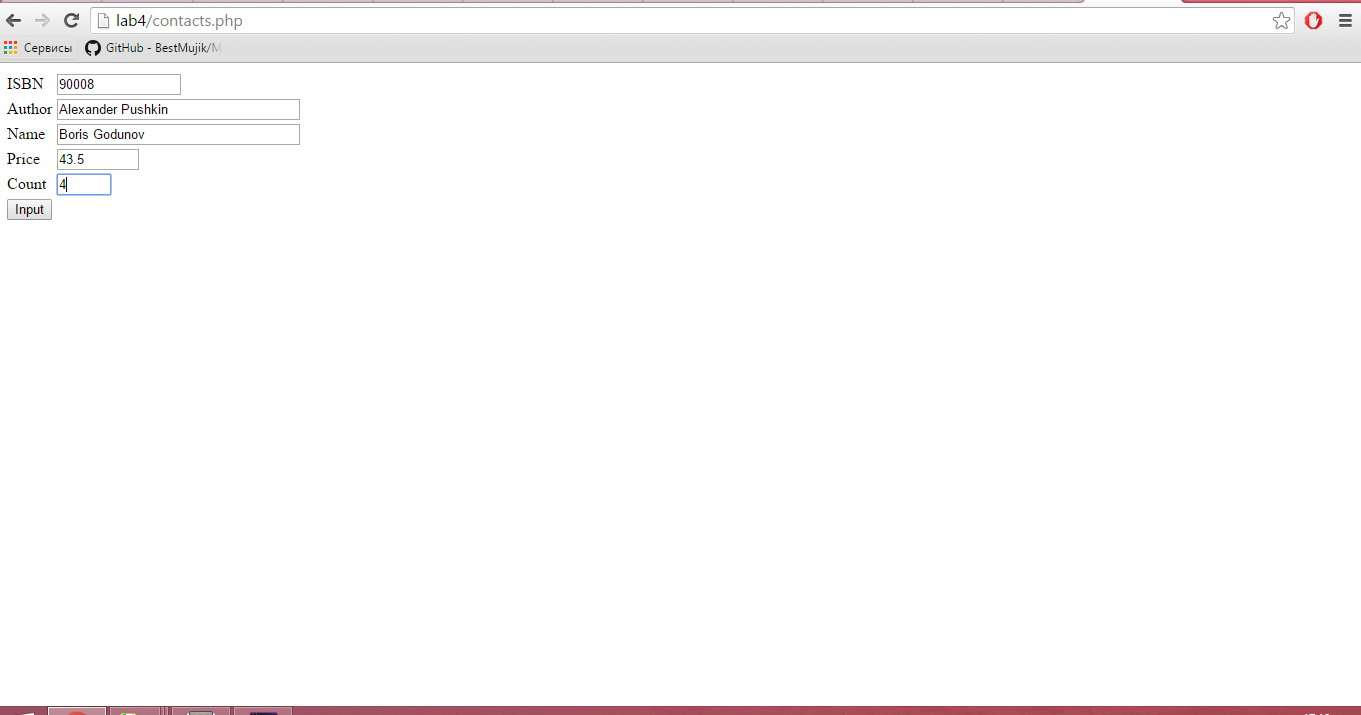
\includegraphics[width=1\linewidth]{images/input.jpg}}
	\caption{Добавленеи книги в БД}
	\label{ris:image}
\end{figure}
\hfill
\begin{figure}[h]
	\center{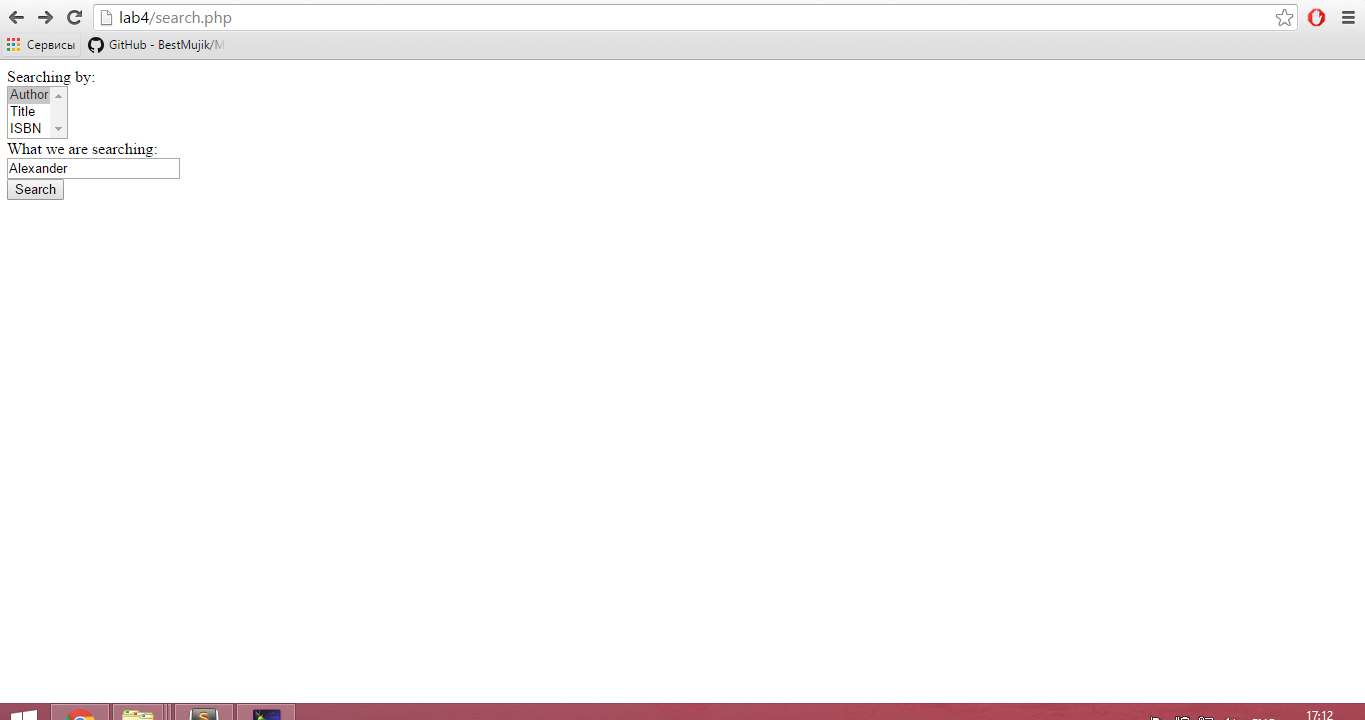
\includegraphics[width=1\linewidth]{images/search.jpg}}
	\caption{Поиск книг в БД}
	\label{ris:image}
\end{figure}
\hfill
\begin{figure}[h]
	\center{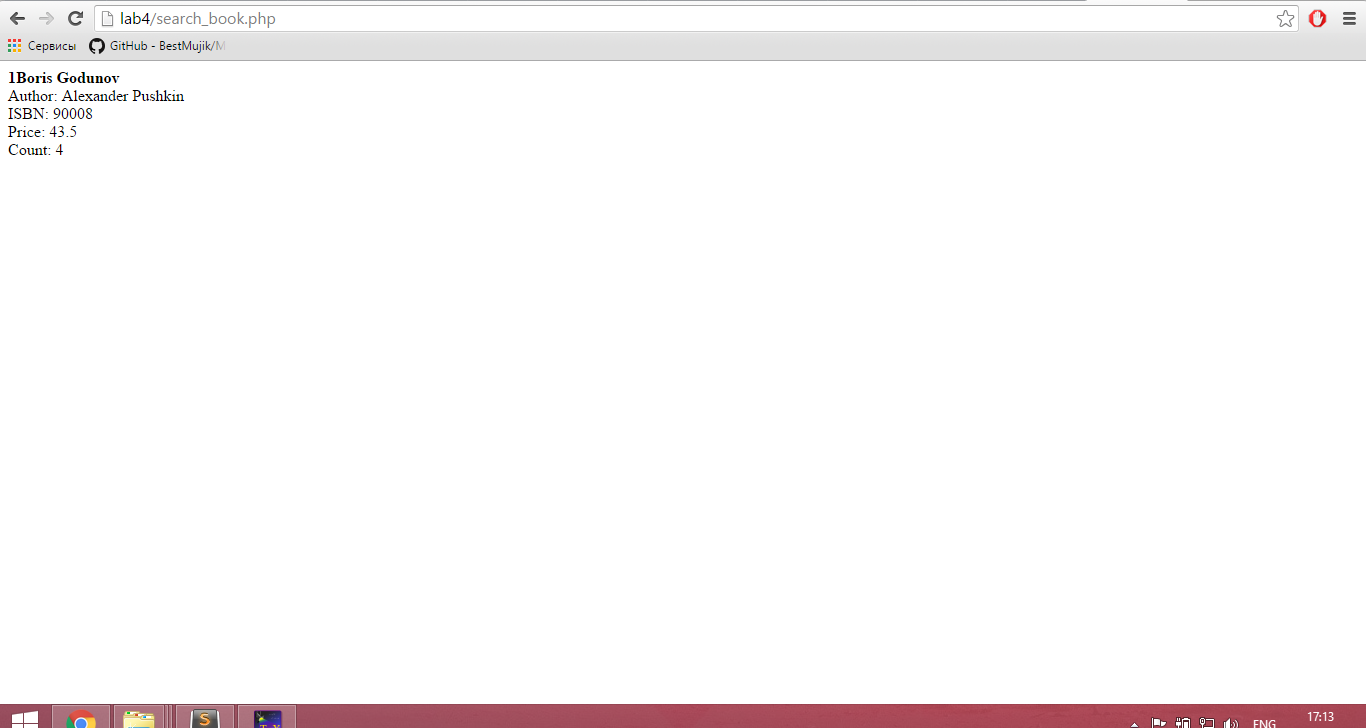
\includegraphics[width=1\linewidth]{images/result.jpg}}
	\caption{Результат поиска}
	\label{ris:image}
\end{figure}

\clearpage